\chapter{Minimum Distance  Estimation}
\section{Minimum Distance Estimator}
In this section we consider a parametric family $\mathcal{F} = \lbrace F_\theta : \theta \in \Theta \subset \mathbb{R}^m \rbrace$, of distribution functions on $\mathbb{R}$, where $\Theta \subset \mathbb{R}^m$ is metric space with Euclidean distance 
\begin{equation}
	\rho (\theta_1,\theta_2) = \sqrt{(\theta_1-\theta_2)(\theta_1-\theta_2)^T}, \quad \theta_1, \, \theta_2 \in \Theta.
\end{equation}
Furthermore, we assume identifiability of the family $\mathcal{F}$, which means 
\begin{equation}
\theta_1 \neq \theta_2 \Rightarrow F_{\theta_1} \neq F_{\theta_2}
\end{equation}
and also that all of $F_\theta(x), \, x \in \mathbb{R}$ are measurable. Our estimators will be calculated on the basis of i.i.d. observations $\mathbf{X}_n = (X_1, \ldots ,X_n)$ all distributed by distribution function $F_{\theta_0} \in \mathcal{F}$. Then $F_{\theta_0} \in \mathcal{F}$ is a true distribution function and $\theta_0 \in \Theta$ is a true parameter.

We are interested in non-parametric estimates of the unknown distribution $F_{\theta_0}$ based on $\mathbf{X}_n$, which are sequences of mappings $ \mathbb{R}^n \rightarrow \mathcal{F}(\mathbb{R}) $ or directly in estimates of the unknown parameter $\theta_0$ (point estimator) based on the same sample $\mathbf{X}_n$, which is sequence of functions $\hat{\theta}_n : \mathbb{R}^n \rightarrow \Theta$. If $\mathcal{F}$ is dominated by a $\sigma$-finite measure $\lambda$ and we write \RN density as
\begin{equation}
f_\theta = \dfrac{\mathrm{d} F_\theta}{\mathrm{d} \lambda},
\end{equation}
we might be also interested in estimator $\hat{f}_n : \mathbb{R}^n \rightarrow \lbrace f_\theta : \theta \in \Theta  \rbrace$ of unknown density $f_{\theta_0}$.

The error of point estimates $\hat{\theta}_n$ is evaluated by $\rho (\hat{\theta}_n,\theta_0)$, error of density estimates by  $\| f_{\hat{\theta}_n} - f_{\theta_0} \|$, where
\begin{equation}
\| f_{\theta_1} - f_{\theta_2} \| = \int{|f_{\theta_1} - f_{\theta_2}|\,\mathrm{d}\lambda}
\end{equation}
is $\mathrm{L}_1$-norm. For evaluating the deviation of distribution functions we need some distance $\mathfrak{D}(F,G) $ on $\mathcal{F}(\mathbb{R}).$

\begin{definition} % 1 
For a set of random variables $X_n$, the notation $X_n = o_p(1)$ means that $\lim_{n \rightarrow \infty } X_n = 0$ holds in probability. The notation $X_n = o_p(\varepsilon_n)$ means that $X_n/\varepsilon_n = o_p(1)$ for some sequence $\varepsilon_n \searrow 0$.
\end{definition} 

\begin{definition} % 2
We say that an estimator $\hat{F}_n$ is {\em consistent estimator} of $F_{\theta_0}$ in distance $\mathfrak{D}$, if $\mathfrak{D}(\hat{F}_n, F_{\theta_0}) = o_p (1)$ and is measurable in $\mathbf{X}_n$.
\end{definition}

%\begin{definition}
%Řekneme, že posloupnost náhodných veličin $\lbrace X_n \rbrace$ s distribučními funkcemi $\lbrace F_n \rbrace$ je omezená v pravděpodobnosti, pokud pro každé $\varepsilon > 0 $ existují $M$ a $N$ takové, že 
%	\begin{equation}
%		F_n(M) - F_n(-M) > 1-\varepsilon, \quad \forall n > N.
%	\end{equation}
%	Tuto skutečnost značíme $X_n = O_p(1)$.
%\end{definition} 

\noindent As an example of non-parametric estimator of cumulative distribution function (CDF) we can use empirical distribution function (ECDF).
\begin{definition}
	Let $(X_1, \ldots,X_n)$ be i.i.d. random sample. Then \emph{empirical distribution function} $F_n(x)$ is defined by 
	\begin{equation}
	F_n(x) = \frac{1}{n} \sum_{i=1}^n I_{X_i \leq x} \quad \forall x \in \mathbb{R},
		\label{eq:ecdf}
	\end{equation}
	where $I_{X_i \leq x}$ is the indicator function defined by 
	\begin{equation}
	I_{X_i \leq x} = 
		\begin{cases}
			1 & \mathrm{if } \: X_i \leq x, \\
			0 & \mathrm{otherwise}.
		\end{cases}		
	\end{equation}
	\label{def:ecdf}	
\end{definition}

\noindent Glivenko-Cantelli theorem states limit property of ECDF:

\begin{theorem}[Glivenko-Cantelli]
	Let $(X_1, \ldots,X_n)$ be i.i.d. random sample with distribution function $F$ and let $F_n(x)$ be ECDF of this sample. Then for all $n \in \mathbb{N}$ it holds, that
	\begin{equation}
	\lim_{n\rightarrow \infty} \sup_{x\in \mathbb{R}} |F(x) - F_n(x)| = 0  \qquad a.s.
	\end{equation}
	\label{theo:glivenko-cantelli}
\end{theorem}
\noindent Proof can be found in \cite{Devroye}.

Later, for analysing FNAL data in chapter \ref{ch:GoF}, we will need weighted empirical distribution function.
\begin{definition}
	Let us have the assumptions from previous definition. Moreover, let us have vector of sample weights $(w_1, \ldots,w_n) \in \mathbb{R}$. Then \emph{weighted empirical distribution function (WECDF)} $F^w_n(x)$ is defined by 
	\begin{equation}
	F^w_n(x) = \frac{1}{W} \sum_{i=1}^n w_i I_{X_i \leq x} \qquad \forall  x \in \mathbb{R},\qquad \text{ where }  W = \sum_{i=1}^n w_i.
	\label{eq:wecdf} 
	\end{equation}	
		\label{def:wecdf}
\end{definition}
%
%\begin{theorem}[Glivenko-Cantelli]
%Nech\v{t} jsou $X_1,\dots,X_n$ stejně a nezávisle rozdělené reálné ná\-ho\-dné veličiny s distribuční funkcí $F$ a nechť $F_n(x)$ je empirická distribuční funkce. Pak pro každé $n\in \mathbb{N}$ a $\varepsilon>0$ platí
%
%\begin{equation}
%P\left(\sup_{x\in\mathbb{R}}|F(x)-F_n(x)|>\varepsilon\right) \leq 8(n+1)\exp{\left\{ \frac{-n{\varepsilon}^2}{32}\right\}}.
%\end{equation}
%Z Borel-Cantelliho lemma pak plyne
%\begin{equation}
%\lim_{n \rightarrow +\infty}\sup_{x \in \mathbb{R}}|F(x)-F_n(x)|=0  \quad \text{s. j.}
%\end{equation}
%\end{theorem}



\noindent Now we can define minimum distance estimator (MDE) and asymptotically minimum distance estimator (AMDE).

\begin{definition}\label{def-mde}
	Let $\mathfrak{D}(\cdot, \cdot) $ be distance on $\mathcal{F}$ and $\hat{F}_n$ an estimator of distribution function $F_{\theta_0}$. A point estimator $\hat{\theta}_n$ measurable in $\Theta$ satisfying the condition
	\begin{equation}
		\mathfrak{D}(\hat{F}_n, F_{\hat{\theta}_n}) = \inf_{\theta \in \Theta}(\hat{F}_n, F_{\theta})
		\label{eq:MDE}
	\end{equation}
	is said to be \emph{minimum distance estimator (MDE)}. If the family $\mathcal{F}$ is dominated by some $\sigma$-finite measure $ \lambda$, then estimator's \RN density $f_{\hat{\theta}_n}$ is said to be \emph{minimum distance probability density estimator}. If the estimator meets the condition
	\begin{equation}
		\mathfrak{D}(F_n, F_{\hat{\theta}_n}) - \inf_{\theta \in \Theta}(F_n, F_{\theta_0}) = o_p(n^{-\frac{1}{2}}), 
	\end{equation}
	 instead of condition \ref{eq:MDE}, the function $\hat{\theta}_n$ is said to be \emph{approximate minimum distance estimator (AMDE)} and the corresponding probability density function $f_{\hat{\theta}_n}$ is said to be \emph{approximate minimum distance probability density estimator}.
\end{definition}

\noindent Note that the rate $n^{-\frac{1}{2}}$ is not important and it can be replaced by any $\varepsilon_n$ tending to 0 sufficiently fast.

\section{Robustness}

Let $\mathcal{P} = \lbrace P_\theta : \theta \in \Theta \subset \mathbb{R}^m \rbrace$ be set of probability distributions on measurable space $\left(\mathcal{X},\mathcal{A}\right)$. Let $T: \mathcal{P} \rightarrow \mathbb{R}^m$ be fisher consistent functional, that means $T(P_\theta) = \theta$ for all $\theta \in \Theta$. We introduce convex mixtures of distributions.

\begin{definition}
	Let us have $\varepsilon \in [0,1]$ and $P, Q \in \mathcal{P}$. We denote convex mixture of distributions $P, Q$ with coefficient $\varepsilon$ by
	\begin{equation}
		P_\varepsilon(Q) = (1-\varepsilon)P + \varepsilon Q.
		\label{konvex-smes}
	\end{equation}
\end{definition}

\subsection{Influence  Function}

Here we define influence function by which we measure the effect of one measurement $x$ on the estimate obtained by functional $T$.

\begin{definition}
	Let $\delta_x$ denotes Dirac delta function at the point $x,\, x \in \mathcal{X}$. \emph{Influence function} $\IF{x}$ of functionals $T \in \mathcal{P},\, P \in \mathcal{P}$, is then defined by
	\begin{equation}
		\IF{x} = \lim_{\varepsilon \rightarrow 0_+} \frac{T(P_\varepsilon(\delta_x)) - T(P)}{\varepsilon} = \lim_{\varepsilon \rightarrow 0_+} \frac{T((1-\varepsilon)P + \varepsilon\delta_x) - T(P)}{\varepsilon}.
	\end{equation} 
\end{definition}

\noindent We can see from the definition, that if $\IF{x}$ is not bounded then even one distant measurement can cause a total failure of the estimator $T$.

We introduce three measures of robustness from \cite{Antoch92}, which characterize some possible disruptions of our model. 

\begin{definition}
	By \emph{gross error sensitivity measure} of functional $T$ for probability distribution $P$ we mean function  $\gamma^*$ defined by 
	\begin{equation}
		\gamma^* = \sup_{x \in \mathcal{X}} |\IF{x}|.
	\end{equation}
\end{definition}
\noindent This function gives a notion of the worst possible effect of occurrence of gross error in data sample on the value of estimator.  From the point of robustness of the estimator, it is therefore desirable for the value of $\gamma^*$ to be finite. Estimators for which the value of $\gamma^*$ is finite are called B-robust.

\begin{definition}
	By \emph{local shift sensitivity measure} of functional $T$ for probability distribution $P$ we mean function  $\lambda^*$ defined by 
	\begin{equation}
			\lambda^* = \sup_{x,y \in \mathcal{X},x \neq y}  \left| \frac{\IF{y} - \IF{x}}{y-x} \right|.
	\end{equation}
\end{definition}

\noindent If the studied probability distribution $P$ is symmetrical w.r.t. point $x=0$, we can define another measure of robustness.

\begin{definition}
	\emph{Rejection point} $\rho^*$ for functional $T$ for probability distribution $P$ is defined by 
	\begin{equation}
			\rho^* = \inf_{x \in \mathcal{X}} \lbrace r>0 \, | \, \IF{x} = 0 \:\; \forall x,\, |x| > r\rbrace.
	\end{equation}
	If such constant $r$  does not exist, we set $\rho^* = + \infty.$ 
\end{definition}

\noindent If the rejection point $\rho^*$ is finite for some estimator, it results from its definition, that contamination of the estimator by measurement in the region  $\lbrace x \, | \, \IF{x} = 0 \rbrace$ does not affect the estimator in any way. If on the other hand the rejection point $\rho^*$ is not finite, it is desirable that at least
\begin{equation}
	\lim_{x \rightarrow \pm\infty} \IF{x} = 0.
\end{equation}

\subsection{\texorpdfstring{$M$}{M}-estimators}
$M$-estimators are generalization of maximum likelihood estimator (MLE). They are estimators defined by maximization or minimization of appropriate function $\rho(\cdot,\cdot):\mathcal{X}\times \Theta \rightarrow \mathbb{R}$. If we have parametric model $\mathcal{P} = \lbrace P_\theta : \theta \in \Theta\rbrace$, then $M$\emph{-estimator} of parameter $\theta$ is defined by 
\begin{equation}
	\hat{\theta}_n = M_n(P_n) = \arg \min_{\theta \in \Theta} \sum_{i=1}^n \rho(X_i,\theta) = \arg \min_{\theta \in \Theta} \mathrm{E}_{P_n}\left[ \rho(X_i,\theta) \right],
	\label{Modhad1}
\end{equation}
where $X_1,\ldots,X_n$ is random sample with probability distribution  $P_\theta$.

If the parametric model has probability density function $p_\theta$, then specific example of M-estimator is MLE which is solution of
\begin{equation}
	\hat{\theta}_{n, MLE} = \arg\min_{\theta \in \Theta} \sum_{i=1}^n \left( -\ln p_\theta(X_i)\right).
\end{equation}

If there exists
\begin{equation}
	\psi(x,\theta) = \frac{\partial}{\partial \theta} \rho(x,\theta), 
\end{equation}
then $M_n$ is the solution, or one of the solutions, of the equation 
\begin{equation}
	\sum_{i=1}^n \psi(X_i,\theta) = 0, \qquad \theta \in \Theta,
	\label{Modhad2}
\end{equation}
so 
\begin{equation}
	\frac{1}{n}\sum_{i=1}^n \psi(X_i,\theta) = \mathrm{E}_{P_n}\left[ \psi(X,\theta) \right] = 0, \qquad \theta \in \Theta.
	\label{Modhad25}
\end{equation}
On the other hand, not every solution of \ref{Modhad2} or \ref{Modhad25} has to be equivalent to solution of \ref{Modhad1}, because some may correspond to one of local maxima.

The functional $M$ which is relevant to $M_n$ is defined by 
\begin{equation}
	M(P) = \arg \min_{\theta \in \Theta} \mathrm{E}_{P}\left[ \rho(x,\theta) \right] = \arg \min_{\theta \in \Theta} \int_\mathcal{X} \rho(x,\theta) \, \mathrm{d}P(x),
	\label{Modhad3}
\end{equation}
or as a solution of equation 
\begin{equation}
\mathrm{E}_{P}\left[ \psi(x,\theta) \right] =  \int_\mathcal{X} \psi(x,\theta) \, \mathrm{d}P(x) = 0, \qquad \theta \in \Theta.
\label{Modhad4}
\end{equation}
For the estimator to be unambiguous, it is required for the equation \ref{Modhad4} or for the minimization \ref{Modhad3} to have a single solution.

Here we present theorem, which allows us to derive influence function for common \ren estimator.
\begin{theorem} 
Let $\psi(\cdot,\theta) =  \frac{\partial}{\partial \theta} \rho(\cdot,\theta)$ exist and let it be absolute continuous with respect to $\theta$. Let equation \eqref{Modhad3} have single solution $M(P)$. Then if it exists, the influence function $\mathrm{IF}(x;M,P)$ is derived by
\begin{equation}
 \text{IF}(x;M,P) = -\left(\int_{\mathcal{X}} \dot{\psi} (y,M(P)) \, \mathrm{d}P(y)\right)^{-1} \psi(x,M(P)),
\end{equation}
where $\dot{\psi} (y,M(P)) = \left[\left(\frac{\mathrm{d}}{\mathrm{d}\theta}\right)^\mathrm{T}\psi(y,\theta)\right]_{\theta = M(P)}$.
\label{theo:IF}
\end{theorem}
\noindent Proof can be found in \cite{Demut2010}.

\section{Decomposable Pseudodistances}

In this section we look into \ren pseudodistance. It will be clear from the following definition, that it is not typical metric distance, because we don't require symmetry nor triangle inequality. 

Let $\mathcal{P} = \lbrace P_\theta : \theta \in \Theta \subset \mathbb{R}^m \rbrace$ be set of probability distributions on measurable space $(\mathcal{X, A})$. Our estimates will be based on i.i.d. observations $\mathbf{X}_n = (X_1, \ldots ,X_n)$ with distribution $P_{0} \in \mathcal{F}$. Because are interested in robustness, we allow $P_{0} \not\in \mathcal{P}$. Therefore we define set $\mathcal{P}^+ = \mathcal{P} \cup \lbrace P_0 \rbrace$.

By $\Pemp$ we denote the class of all empirical distribution functions, not necessarily from $\mathcal{P}.$
		
		\begin{definition}
	We say that the mapping $\mathfrak{D}:\mathcal{P}\times\mathcal{P}^+ \rightarrow \mathbb{R}$ is a \emph{pseudodistance} between probability measures $P \in \mathcal{P}$ and $Q \in \mathcal{P}^+$ if it holds, that	
		\begin{equation}
			\mathfrak{D}(P_\theta,Q) \geq 0 \qquad \forall \theta \in \Theta, \: \forall Q \in \mathcal{P}^+
		\end{equation}
		and 		
		\begin{equation}
			\mathfrak{D}(P_{\theta_1},P_{\theta_2})=0 \; \Leftrightarrow \; \theta_1=\theta_2 \qquad \forall \theta_1,\: \theta_2 \in \Theta.
		\end{equation}	
	This pseudodistance $\mathfrak{D}$ is called \emph{decomposable} on $\mathcal{P}\times\mathcal{P}^+$ if there exist functionals 
		 $\mathfrak{D}^0:\mathcal{P}\rightarrow\mathbb{R}$, $ \mathfrak{D}^1:\mathcal{P}^+ \rightarrow \mathbb{R}$ and measurable mapping
		  $\rho_\theta : \mathbb{R}^d \rightarrow \mathbb{R}$, $ \theta \in \Theta$, so that for all $\theta \in \Theta$ and for all $Q \in \mathcal{P}^+$ the expectation $\int{\rho_\theta }\, \mathrm{d}Q$ exists and it holds, that
		\begin{equation}
			\mathfrak{D} (P_\theta, Q) = \mathfrak{D}^0 (P_\theta) + \mathfrak{D}^1 (Q) + \int \rho_\theta \, \mathrm{d}Q.
		\end{equation}
\end{definition}

\begin{definition}
	We say that a functional $T_\mathfrak{D}:\mathcal{Q} \rightarrow \Theta$, for $\mathcal{Q}=\mathcal{P}^+ \cup \mathcal{P}_{\text{emp}}$	defines \emph{minimum pseudodistance estimator} (min $\mathfrak{D}$-estimator) if $\mathfrak{D}(P_\theta,Q)$ is a decomposable pseudodistance on $\mathcal{P}\times\mathcal{P}^+$ and parameters $T_\mathfrak{D}(Q) \in \Theta$ minimize $\mathfrak{D}^0 + \int{\rho_\theta}\,\mathrm{d}Q$ on $\Theta$ for all $Q \in \mathcal{Q}$, that means
	\begin{equation}
		T_\mathfrak{D}(Q) = \arg\min_{\theta \in \Theta} \left[ \mathfrak{D}^0(P_\theta) + \int{\rho_\theta}\,\mathrm{d}Q \right] \quad \forall Q \in \mathcal{Q}.
	\end{equation}
\end{definition}
\noindent In particular, for the empirical distribution function $Q = P_n = \frac{1}{n}\sum_{i-1}^n \delta_{X_i} \in \mathcal{P}_{emp}$
\begin{equation}
	\hat{\theta}_{\mathfrak{D},n} =T_\mathfrak{D}(P_n)  = \arg\min_{\theta \in \Theta}\left[ \mathfrak{D}^0(P_\theta) + \dfrac{1}{n} \sum_{i=1}^n \rho_\theta (X_i) \right].
\end{equation}
\begin{theorem}
	Every min $\mathfrak{D}$-estimator 
	\begin{equation}
		\left[ \mathfrak{D}^0(P_\theta) + \dfrac{1}{n} \sum_{i=1}^n \rho_\theta (X_i) \right]
	\end{equation}
	is Fisher consistent in the sense that
\begin{equation}
	T_\mathfrak{D}(P_{\theta_0}) = \arg\min_{\theta \in \Theta} \mathfrak{D}(P_\theta, P_{\theta_0}) = \theta_0,\quad \forall \theta_0 \in \Theta.
\end{equation}
\end{theorem}
\begin{proof}
Consider any fixed $\theta_0 \in \Theta$. Then $\mathfrak{D}^1(P_{\theta_0})$ is finite constant and from the definition of pseudodistance we get
\begin{align*}
T_\mathfrak{D}(P_{\theta_0}) & = \arg\min_{\theta \in \Theta} \left[ \mathfrak{D}^0(P_\theta) + \int{\rho_\theta}\,\mathrm{d}Q \right] 
% & = \arg\min_{\theta \in \Theta} \left[ \mathfrak{D}^0(P_\theta) +\mathfrak{D}^1(P_{\theta_0}) + \int{\rho_\theta}\,\mathrm{d}Q \right] 
 = \arg\min_{\theta \in \Theta} \mathfrak{D}(P_\theta,P_{\theta_0}) 
= \theta_0.
\end{align*}
\end{proof}


\begin{theorem}
Let for some $\beta>0$ it holds that
	\begin{equation}
			p^\beta, q^\beta,\ln{p} \in \mathrm{L}_1(Q), \quad \forall P \in \mathcal{P}, Q \in \mathcal{P^+}.
			\label{eq:betaCond}
	\end{equation}
	Then for all $\alpha$, $0 < \alpha \leq \beta$, and for $P \in \mathcal{P}, \; Q \in \mathcal{P^+} $ the expression
	\begin{equation}
		\mathfrak{R}_\alpha (P,Q) = \dfrac{1}{1+\alpha}\ln{\left( \int{p^\alpha \,\mathrm{d}P } \right)} +
		\dfrac{1}{\alpha (1+\alpha)}\ln{\left( \int{q^\alpha \,\mathrm{d}Q } \right)} -
		\dfrac{1}{\alpha} \ln{\left( \int{p^\alpha \,\mathrm{d}Q } \right)}
		\label{eq:renDecDist}
	\end{equation}
		represents the family of pseudodistances decomposable in the sense of
	\begin{equation*}
		\mathfrak{R}_\alpha (P,Q) = \mathfrak{R}_\alpha^0 (P) + \mathfrak{R}_\alpha^1 (Q) - \dfrac{1}{\alpha} \ln{\left( \int{p^\alpha \,\mathrm{d}Q } \right)},
	\end{equation*}	
	where
	\begin{equation*}
		\mathfrak{R}_\alpha^0 (P) = \dfrac{1}{1+\alpha}\ln{\left( \int{p^\alpha \,\mathrm{d}P } \right)}, \quad \mathfrak{R}_\alpha^1 (Q) = \dfrac{1}{\alpha (1+\alpha)}\ln{\left( \int{q^\alpha \,\mathrm{d}Q } \right)}.
	\end{equation*}
	Moreover, for $\alpha \searrow 0$ it holds
	\begin{equation*}
		\mathfrak{R}_0 (P,Q) = \lim_{\alpha \searrow 0} \mathfrak{R}_\alpha (P,Q) =  \int{\left( \ln{q} - \ln{p} \right)\,\mathrm{d}Q}.
	\end{equation*}
\end{theorem}
\noindent Proof can be found in \cite{Decomposable2011}. \\
If we use \ref{eq:renDecDist} for distributions $Q \in \mathcal{P}^+ \cup \Pemp$ we get minimum \ren distance estimator defined by

\begin{equation}
	T_{\mathfrak{R}_\alpha}(Q) =
	\begin{cases}
		 \arg \min_{\theta} \left[\frac{1}{1+\alpha} \ln(\int p_\theta^\alpha\, \mathrm{d}P_\theta) - \frac{1}{\alpha} \ln(\int p_\theta^\alpha\, \mathrm{d}Q) \right] & \text{if } 0 < \alpha \leq \beta, \\
		 \arg \min_{\theta} \left[- \ln(\int p_\theta\, \mathrm{d}Q) \right] & \text{if } \alpha = 0,
	\end{cases}	
\end{equation}
which is equivalent to 
\begin{equation}
	T_{\mathfrak{R}_\alpha}(Q) = 
	\begin{cases}
		 \displaystyle{ \arg \max_{\theta \in \Theta} \left[\ln\frac{\int p_\theta^\alpha\, \mathrm{d}Q}{(\int p_\theta^\alpha\, \mathrm{d}P_\theta)^{\frac{\alpha}{1+\alpha}}} \right] }& \text{ if } 0 < \alpha \leq \beta, \\[5mm]
		 \displaystyle{ \arg \max_{\theta \in \Theta} \left[\ln(\int p_\theta\, \mathrm{d}Q) \right] }& \text{ if } \alpha = 0.
	\end{cases}	
\end{equation}
If we denote
\begin{equation}
C_{\alpha}(\theta) = \biggl(\int p_{\theta}^{1+\alpha} \, \mathrm{d}\lambda\biggr)^{\frac{\alpha}{1+\alpha}} = \left( \int p_\theta^\alpha\, \mathrm{d}P_\theta \right)^{\frac{\alpha}{1+\alpha}},
\end{equation}
then we can write \ren estimator for $0<\alpha \leq \beta$ in the form of $M$-estimator
\begin{equation}
T_{\alpha}(Q) = \text{argmax}_{\theta} M_{\alpha}(Q,\theta), \qquad \text{where } \quad M_{\alpha}(Q,\theta) = \frac{\int p_{\theta}^{\alpha}\, \mathrm{d}Q}{C_{\alpha}(\theta)}.
\end{equation}

We are interested in estimators, in which we replace the hypothetical distribution $P_{\theta_0}$ in $\mathfrak{R}_\alpha(P_\theta, P_{\theta_0})$ by empirical distribution $P_n \in \Pemp$. In this case we can write minimum \ren distance estimator in the form

% It means that the family of minimum \ren pseudo-distance estimators defined by $\hat{\theta}_{n,\alpha} = T_{\mathfrak{R}_\alpha}(P_n)$ for $T_{\mathfrak{R}_\alpha}(Q) \in \Theta$ with $Q \in \mathcal{P}^+$ satisfies the condition

\begin{equation}
	\hat{\theta}_{\mathfrak{R}_\alpha,n} =
	\begin{cases}
		\displaystyle{ \arg \max_{\theta \in \Theta} C_\alpha\left( \theta \right)^{-1} \frac{1}{n} \sum_{i=1}^n p_{\theta}^{\alpha}\left( X_i \right) } & \text{if } 0 < \alpha \leq \beta, \\
		\displaystyle{ \arg \max_{\theta \in \Theta}  \frac{1}{n} \sum_{i=1}^n \ln p_{\theta}\left( X_i \right) } & \text{if } \alpha = 0.
	\end{cases}	
	\label{eq:renEstimator}
\end{equation}
In \cite{Vajda2009} author derives form of influence function for minimum \ren pseudodistance estimator according to theorem \ref{theo:IF}. If we use notation 
\begin{center}
	\begin{tabular}{c c}
	$s_\theta = \dfrac{\mathrm{d}}{\mathrm{d}\theta} \ln p_\theta, \quad$ & $ \dot{s}_\theta = \left( \dfrac{\mathrm{d}}{\mathrm{d}\theta} \right)^T s_\theta,$ \\ 
	&\\
	$c_\alpha(\theta) = \dfrac{\int p_\theta^{1+\alpha}s_\theta \mathrm{d}\lambda}{\int p_\theta^{1+\alpha} \mathrm{d}\lambda}, \quad$ & $\dot{c}_\alpha(\theta)= \left( \dfrac{\mathrm{d}}{\mathrm{d}\theta} \right)^T c_\alpha(\theta),$  \\ 
	\end{tabular} 
\end{center}
then the influence function can be written by
\begin{equation}
	\mathrm{IF}(x;T_{\mathfrak{R}_\alpha},\theta) = -\mathbf{I}^{-1}_{\alpha}(\theta) \left[ p_\theta^\alpha(x) (s_\theta (x) - c_\alpha (x)) \right], 
	\label{eq:IF}
\end{equation}
where 
\begin{equation}
\mathbf{I}_{\alpha}(\theta) = \int{ \left[\dot{s}_\theta - \dot{c}_\alpha(\theta) - \alpha(s_\theta - c_\alpha(\theta))(c^T_\alpha(\theta) - s^T_\theta) \right] p_\theta^{1+\alpha} \mathrm{d}\lambda}.
\end{equation}

\subsection{Applications for Normal Distribution}

Results for normal model including specific forms of estimator \eqref{eq:renEstimator} and influence function \eqref{eq:IF} were already presented in \cite{Vajda2009} and \cite{Demut2010}. We are presenting them here for completeness and because we used them in simulations in which we tested the estimators on data samples with different kind of contamination from what was used in \cite{Demut2010}. 

Minimum \ren distance estimator for $\alpha = 0$ coincides with maximum likelihood estimator
\begin{equation}
\hat{\theta}_{\mathfrak{R}_0,n} = \text{argmax}_{\theta} \frac{1}{n}\sum_{i=1}^n \ln \biggl[\frac{1}{\sqrt{2\pi \sigma^2}} \exp\biggl(-\frac{(X_i-\mu)^2}{2\sigma^2}\biggr)\biggr].
\end{equation}

\noindent Condition\ref{eq:betaCond} holds for all $\beta > 0$, therefore for $\alpha>0$ we can transform {\mRao} \eqref{eq:renEstimator} to

\begin{equation}
	\hat{\theta}_{\mathfrak{R}_\alpha,n} = \text{argmax}_{\theta} \frac{1}{n\sigma^{\alpha/(1+\alpha)}}\sum_{i=1}^n\exp \biggl(-\alpha\frac{(X_i-\mu)^2}{2\sigma^2}\biggr).
\end{equation}

\noindent Influence function for estimator of the standard deviation $\sigma$ with the known mean $\mu = 0$ is derived in \cite{Vajda2009} and has the form

\begin{equation}
	\text{IF}(x;T_{\mathfrak{R}_{\alpha}},\sigma) = \frac{(1+\alpha)^{5/2}\sigma}{2}\biggl[\biggl(\biggl(\frac{x}{\sigma}\biggr)^2-\frac{1}{1+\alpha}\biggr) \exp\biggl(-\frac{\alpha x^2}{2\sigma^2}\biggr)\biggr].
\end{equation}
For the estimator of mean $\mu$ with fixed $\sigma$ the influence function takes the form
\begin{equation}
	\text{IF}(x;T_{\mathfrak{R}_{\alpha}},\mu) = (1+\alpha )^{3/2} (x-\mu ) \exp\left[{-\alpha\frac{(x-\mu )^2}{2 \sigma ^2}}\right].
\end{equation}
Both functions are bounded for all possible $\alpha$, which means that the estimator is B-robust. Although we do not have finite rejection point $\rho^*$, we can see, that for $\alpha>0$ the limit 
\begin{equation}
	\lim_{x \rightarrow \pm\infty} \mathrm{IF}(x;T_{\mathfrak{R}_\alpha},\cdot) = 0
\end{equation}	
holds for influence functions for both parameters.	
	
	\section{Application to Specific Families}
	
In this section we will use \mRa-estimators for some specific families of probability distributions. As was stated above, results for normal model were already presented in  \cite{Vajda2009}, \cite{Demut2010}. Therefore we focused on exponential, Laplace, Cauchy and Weibull families. In case of these families we focused on deriving specific simple forms of estimator according to \eqref{eq:renEstimator} and also the form of influence function \eqref{eq:IF}.

\subsection{Laplace distribution} 
Here we use \mRa-estimators to estimate parameter $\theta = (\mu,\lambda)$ in Laplace model. Laplace probability density function can be written as 
\begin{equation}
	p_\theta = \frac{1}{2\lambda} e^{-\frac{|x-\mu|}{\lambda}}, \qquad \mu\in \mathbb{R},\, \lambda>0.
\end{equation}
For $\alpha = 0$ is the estimator \eqref{eq:renEstimator} equal to maximum likelihood estimator
\begin{align}
	\hat{\theta}_{\mathfrak{R}_0,n} & = \arg \max_{\theta \in \Theta} \frac{1}{n} \sum^n_{i=1} \ln \left[ \frac{1}{2\lambda}\exp \left[-\frac{|x_i-\mu|}{\lambda} \right] \right] \nonumber \\
	& =  \arg \max_{\theta \in \Theta} \left[ \ln \frac{1}{2\lambda} - \frac{1}{n} \sum^n_{i=1} \frac{|x_i-\mu|}{\lambda} \right].
\end{align}
Condition \eqref{eq:betaCond} holds for all $\beta>0$, therefore we can \mRa-estimator \eqref{eq:renEstimator} of parameters of Laplace distribution write for $\alpha>0$ as
\begin{equation}
	\hat{\theta}_{\mathfrak{R}_\alpha,n} = \arg \max_{\theta \in \Theta} \left[ (2\lambda)^{-\frac{\alpha}{1+\alpha}} \frac{1}{n} \sum_{i=1}^n \exp \left[-\alpha\frac{|x_i-\mu|}{\lambda} \right] \right].
	\label{renyi-formula-laplace}
\end{equation}
Via this formula we can estimate simultaneously both parameters $\mu, \lambda$ of the model. If one of the parameters is known and therefore there isn't need for it's estimation, we can simply fix it's value and maximize over the second parameter.

Here we present influence function for \mRa-estimator for Laplace model calculated from \eqref{eq:IF}. For the location estimator $(\hat{\theta} = \mu)$ with$\lambda$ known, we get influence function in the form

\begin{equation}
	\mathrm{IF}(x;T_{\mathfrak{R}_\alpha},\mu) = (1+\alpha )^{\frac{3}{2}} (x-\mu )  e^{-\frac{\alpha}{2} (x-\mu )^2}. % IF(x,mu)
	\label{IF-laplace-mu}
\end{equation}
If we switch the role of the parameters, meaning that we estimate the scale $\hat{\theta} = \lambda$, while fixing the $ \mu$, we get 
\begin{equation}
	\mathrm{IF}(x;T_{\mathfrak{R}_\alpha},\lambda) = (1 + \alpha)^2 \left(-\lambda + (1 + \alpha)|x-\mu|\right)  e^{-\frac{\alpha|x-\mu|}{\lambda}}	. % IF(x,sigma)
	\label{IF-laplace-lambda}
\end{equation}

\begin{figure}[htb]
\begin{center}
\begin{tabular}{c c c}
	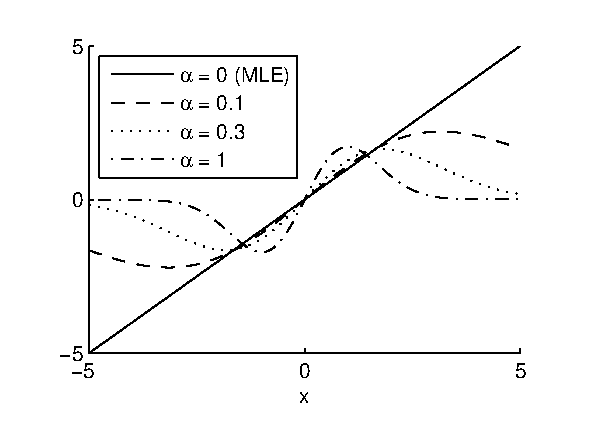
\epsfig{file=Laplace-IF-mu.eps, height=2.in} 
	&&
	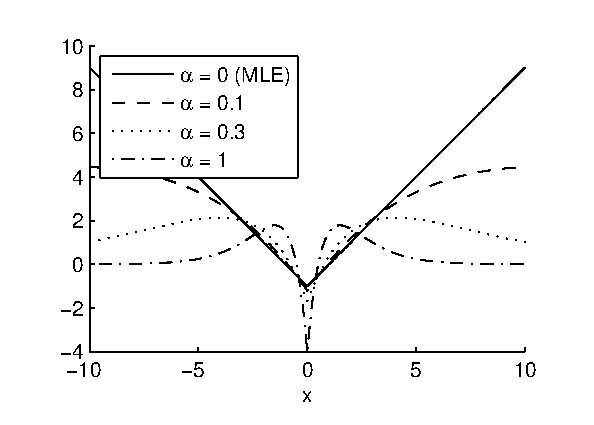
\epsfig{file=Laplace-IF-lambda.eps, height=2.in} 
	\\
	$\mathrm{IF}(x;T_{\mathfrak{R}_\alpha},\mu = 0) $ in case of known $\lambda = 1$ 
	&&
	$\mathrm{IF}(x;T_{\mathfrak{R}_\alpha},\lambda = 1)$ in case of known $\mu = 0$ 
	\\
\end{tabular}
\caption{Influence function of \mRa-estimators of parameters of Laplace distribution}
\label{fig:laplace-if}
\end{center}
%\label{fig:laplace-if}
\end{figure}

From \eqref{IF-laplace-mu} and \eqref{IF-laplace-lambda} we can see, that both influence functions are for $\alpha>0$ bounded, therefore B-robust. 

Moreover for both functions it holds that 

\begin{equation}
	\lim_{x \rightarrow \pm\infty} \mathrm{IF}(x;T_{\mathfrak{R}_\alpha},\cdot) = 0.
\end{equation}
 
\noindent Although the rejection points $\rho^*$ isn't finite, but the limits hold. We can see, that this convergence has exponential development in $\alpha$ due to the component  $e^{-\alpha x}$ in both functions. This means, that the estimator is more robust with higher value of $\alpha$. This can be also seen in the figure \ref{fig:laplace-if}, where the influence functions for both estimated parameters are shown separately for various $\alpha$.  We can see that maximum likelihood estimator $(\alpha = 0)$ isn't bounded and that the functions approach 0 faster with increasing $|x|$ for higher values of $\alpha$.

\subsection{Exponential distribution} 
Here we use \mRa-estimators to estimate parameter $\theta = (\mu,\lambda)$ in exponential distribution with probability density function 
\begin{equation}
	p_\theta = \frac{1}{\lambda} e^{-\frac{x-\mu}{\lambda}}, \qquad \mu\in \mathbb{R},\, \lambda>0, \, x\geq\mu.
\end{equation}
\noindent Exponential density's form is very similar to that of Laplace density. Below we will see, that even formulas for \mRa-estimators are very similar in both models. For $\alpha = 0$ we get \mRa-estimator in the form
\begin{align}
	\hat{\theta}_{\mathfrak{R}_0,n} & =  \arg \max_{\theta \in \Theta} \frac{1}{n} \sum^n_{i=1} \ln \left[ \frac{1}{\lambda}\exp \left[-\frac{x_i-\mu}{\lambda} \right] \right] \nonumber \\
	& =  \arg \max_{\theta \in \Theta} \left[ \ln \frac{1}{\lambda} - \frac{1}{n} \sum^n_{i=1} \frac{x_i-\mu}{\lambda} \right].
\end{align}

\noindent Condition \ref{eq:betaCond} holds again for all  $\beta>0$, therefore we can write \mRa-estimator for exponential family for $\alpha>0$ as
\begin{equation}
	\hat{\theta}_{\mathfrak{R}_\alpha,n} = \arg \max_{\theta \in \Theta} \lambda^{-\frac{\alpha}{1+\alpha}} \frac{1}{n}\sum_{i=1}^n \exp \left[-\alpha\frac{x_i-\mu}{\lambda} \right].
	\label{renyi-formula-exponential}
\end{equation}

We can see, that the difference to \eqref{renyi-formula-laplace} is only in the use of absolute value in Laplace model.

For  the estimator of location $\hat{\theta} = \mu$ in case of known $\lambda$, the influence function is the same as in the Laplace family $\eqref{IF-laplace-mu}$, therefore it holds

\begin{equation}
	\mathrm{IF}(x;T_{\mathfrak{R}_\alpha},\mu) = (1+\alpha )^{\frac{3}{2}} (x-\mu )  e^{-\frac{\alpha}{2} (x-\mu )^2}. % IF(x,mu)
	\label{IF-exponential-mu}
\end{equation}
If we estimate parameter of scale $\hat{\theta} = \lambda$ in case of known $ \mu $, we get formula
\begin{equation}
	\mathrm{IF}(x;T_{\mathfrak{R}_\alpha},\lambda) =	(1+\alpha )^2 \left( - \lambda +(1+ \alpha)(x-\mu)\right) e^{-\frac{\alpha (x-\mu)}{\lambda }}. % IF(x,lambda),
	\label{IF-exponential-lambda}
\end{equation}

\begin{figure}[htb]
\begin{center}
\begin{tabular}{c c c}
	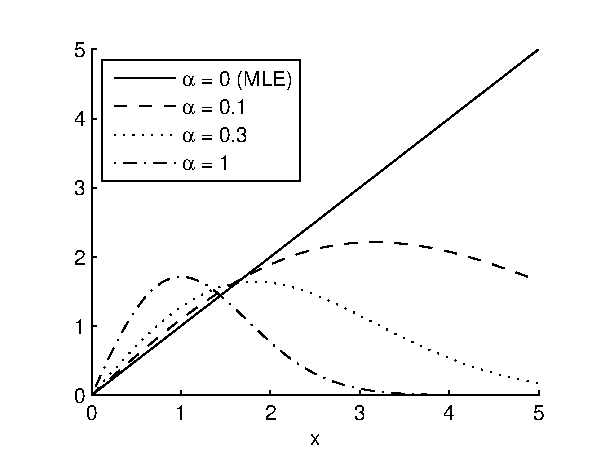
\epsfig{file=Exp-IF-mu.eps, height=2.1in} 
	&&
	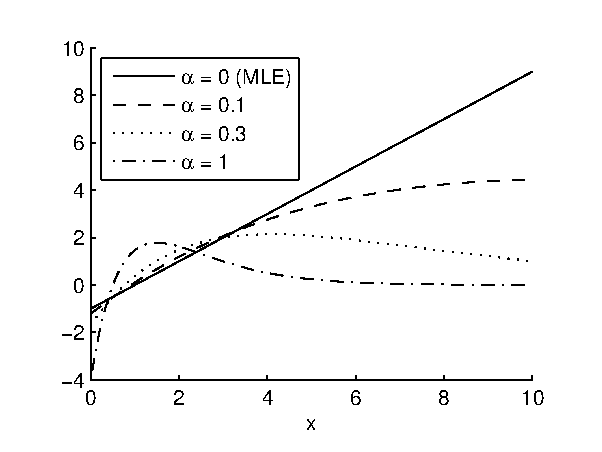
\epsfig{file=Exp-IF-lambda.eps, height=2.1in} 
	\\
	$\mathrm{IF}(x;T_{\mathfrak{R}_\alpha},\mu = 0) $ in case of known $\lambda = 1$
	&&
	$\mathrm{IF}(x;T_{\mathfrak{R}_\alpha},\lambda = 1)$ in case of known $\mu = 0$
	\\
\end{tabular}
\caption{Influence function of \mRa-estimators of parameters of exponential distribution}
\label{fig-exp-if}
\end{center}
\end{figure}

\noindent We can see from \eqref{IF-exponential-mu} and \eqref{IF-exponential-lambda} that for both functions it holds, that

\begin{equation}
	\lim_{x \rightarrow \pm\infty} \mathrm{IF}(x;T_{\mathfrak{R}_\alpha},\cdot) = 0,
\end{equation}
therefore outliers will be partially ignored due to the convergence of influence functions to 0. Again it holds, that the convergence is faster with greater $\alpha$, which can be seen in figure \ref{fig-exp-if}, as well as the fact, that the functions are bounded for all $\alpha >0$.

\subsection{Cauchy distribution} 


Dalším rozdělením, na které jsme použili Rényiho odhady, je Cauchyho s parametrem $\theta = (\mu,\sigma)$ a hustotou pravděpodobnosti
\begin{equation}
	p_\theta = \frac{1}{\pi\sigma} \left( 1 + \left( \frac{x-\mu}{\sigma} \right)^2 \right)^{-1}, \qquad \mu\in \mathbb{R},\, \sigma>0.
\end{equation}
Minimální $\mathfrak{R}_\alpha$-odhad je pro $\alpha=0$ roven
\begin{align}
	\hat{\theta}_{\mathfrak{R}_0,n} & = \arg \max_{\theta \in \Theta} \frac{1}{n} \sum^n_{i=1} \ln \left[  \frac{1}{\pi\sigma} \left( 1 + \left( \frac{x_i-\mu}{\sigma} \right)^2 \right)^{-1}   \right] \nonumber \\
	& =  \arg \max_{\theta \in \Theta} \left[ -\ln \pi\sigma - \frac{1}{n} \sum^n_{i=1} \ln \left[ 1 + \left( \frac{x_i-\mu}{\sigma} \right)^2 \right] \right],
\end{align}
který je shodný s maximálně věrohodným odhadem. Podmínka \eqref{eq:betaCond} platí tak jako v předchozích případech pro každé $\beta>0$. Pro $\alpha>0$ pak vychází minimální $\mathfrak{R}_\alpha$-odhad \eqref{eq:renEstimator} parametrů v Cauchyho modelu jako 

\begin{equation}
	\hat{\theta}_{\mathfrak{R}_\alpha,n} = \arg \max_{\theta \in \Theta} \left[ \sigma^{-\frac{\alpha}{1+\alpha}} \frac{1}{n} \sum_{i=1}^n \left( 1 + \left( \frac{x_i-\mu}{\sigma} \right)^2 \right)^{-\alpha} \right].
	\label{renyi-formula-cauchy}
\end{equation}

Influenční funkci \eqref{IF} pro minimální $\mathfrak{R}_\alpha$-odhady v Cauchyho rodině se nám podařilo dopočítat jen pro odhad parametru polohy $\theta = \mu$. Za předpokladu znalosti měřítka $\sigma$ má funkce tvar

\begin{equation}
	\mathrm{IF}(x;T_{\mathfrak{R}_\alpha},\mu) = \sqrt{\pi}\frac{\Gamma\left( 3 + \alpha \right)}{\Gamma\left( \frac{3}{2} + \alpha \right)} \left( \frac{\sigma^2}{\sigma^2 + (x-\mu)^2}\right)^{1+\alpha}(x-\mu).
	\label{IF-cauchy-mu}
\end{equation}

\noindent Z \eqref{IF-cauchy-mu} a obrázku \ref{fig:cauchy-if} je vidět, že influenční funkce je pro $\alpha>0$ omezená. Bod zamítání $\rho^*$ opět není konečný, ale pro $\alpha>0$ platí alespoň limita

\begin{equation}
	\lim_{x \rightarrow \pm\infty} \mathrm{IF}(x;T_{\mathfrak{R}_\alpha},\mu) = 0.
\end{equation}

\begin{figure}[htb]
\begin{center}
\begin{tabular}{c}
	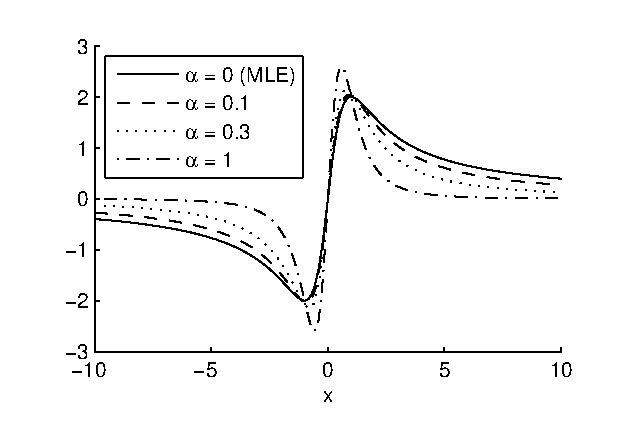
\epsfig{file=Cauchy-IF-mu.eps, height=2.6in} \\
	$\mathrm{IF}(x;T_{\mathfrak{R}_\alpha},\mu = 0) $ při $\sigma = 1$ známém
\end{tabular}
\caption{Influenční funkce {\mRao}ů pro Cauchyovo rozdělení}
\label{fig:cauchy-if}
\end{center}
\end{figure}

\noindent Podle vzorce \eqref{IF} se  nakonec podařilo dopočítat influenční funkci pro odhad měřítka $\theta = \sigma$ při znalosti polohy $\mu$. Následujícího výsledku bylo dosaženo výpočtem ve \texttt{Wolfram Mathematica}. Výsledný tvar je tedy

\begin{eqnarray}
\mathrm{IF}(x;T_{\mathfrak{R}_\alpha},\sigma) &=& -\left[4 \sqrt{\pi } (1+\alpha )^2 \sigma ^{2+\alpha } \left(\frac{\sigma }{(x-\mu )^2+\sigma ^2}\right)^{\alpha} \right. \nonumber\\
&&\left(\frac{1}{\sigma }+\frac{\alpha  \left(\frac{1}{\sigma }\right)^{\alpha } \sigma ^{-1+\alpha }}{1+\alpha }-\frac{2 \sigma }{(x-\mu )^2+\sigma ^2}\right) \left. \cos[\pi  \alpha ] \Gamma[\alpha ] \Gamma[1+\alpha ]  \frac{}{} \right] / \nonumber \\ %prázdný zlomek je tam kvůli roztažení koncové závorky
&&\left(4^{1-\alpha } \sqrt{\pi } \left(\frac{1}{\sigma }\right)^{\alpha } \sigma ^{\alpha } \left(-1+\alpha  \left(-1+\alpha  \left(-2+\left(\frac{1}{\sigma }\right)^{\alpha } \sigma ^{\alpha }\right)\right)\right) \right.\nonumber \\ 
&&\left. \cos[\pi  \alpha ] \Gamma[1+2 \alpha ]+1/(3 (3+4 \alpha  (2+\alpha )))\right. \nonumber \\
&& 8 \pi  (1+\alpha ) \left(-1+\alpha  (1+\alpha )^2\right) \Gamma[\alpha ] \nonumber \\
&& \left(6 (1+\alpha ) ^r_2\mathrm{F}_1\left[\frac{1}{2},2,\frac{1}{2}-\alpha ,1\right]-4^{-\alpha } \Gamma[4+2 \alpha ] \right. \nonumber \\
&& \left. \left. ^r_2\mathrm{F}_1\left[\frac{1}{2}+\alpha ,1+\alpha ,-\frac{1}{2}+\alpha ,1\right]\right)\right),
\end{eqnarray}

\noindent kde $^r_2\mathrm{F}_1[a,b;c;z]$ je regularizovaná hypergeometrická funkce 

\begin{equation}
	^r_2\mathrm{F}_1[a,b;c;z] = {\frac{1}{\Gamma[c]}} {_2\mathrm{F}_1}[a,b;c;z],
\end{equation}
přičemž hypergeometrická funkce je definovaná vztahem
\begin{equation}
	{_2\mathrm{F}_1}[a,b;c;z]=\sum _{n=0}^{\infty } \frac{(a)_n (b)_n z^n}{ (c)_n n!}, \qquad |z|<1, \, \text{ nebo } \, (|z|=1\l  \,\text{a} \,  c>a+b),
\end{equation}

\noindent kde $(a)_n$ je Pochhammerův symbol definovaný

\begin{equation}
(a)_n=\prod _{k=0}^{n-1} (a+k), \qquad n \in \mathbb{N}.
\end{equation}

\noindent Kvůli definici hypergeometrické funkce tato influenční funkce však nemá smysl, protože z definičních podmínek nám vychází $\frac{1}{2}+\alpha  + 1+\alpha < -\frac{1}{2}+\alpha $, tedy $\alpha < -2$, což ale odporuje výběru $\alpha>0$ z věty \ref{renyi-veta}. 

\subsection{Weibull distribution} 

Posledním zpracovávaným rozdělením, bylo tříparametriké Weibullovo s parametrem $\theta = (\mu,\lambda,k)$ a hustotou pravděpodobnosti
\begin{equation}
	p_\theta =  \frac{k}{\lambda} \left( \frac{x-\mu}{\lambda} \right)^{k-1} \exp \left[ -\left( \frac{x-\mu}{\lambda} \right)^k \right], \qquad \mu \in \mathbb{R}, \, \lambda>0, \, k>0, \, x \geq \mu.
\end{equation}

\noindent Pro $\alpha = 0$ je minimální Rényiho odhad roven

\begin{align}
	\hat{\theta}_{\mathfrak{R}_0,n} & = \arg \max_{\theta \in \Theta} \frac{1}{n} \sum^n_{i=1} \ln \left[ \frac{k}{\lambda} \left( \frac{x_i-\mu}{\lambda} \right)^{k-1} 
	\exp \left[ -\left( \frac{x_i-\mu}{\lambda} \right)^k \right]\right] \nonumber \\
	&=\arg \max_{\theta \in \Theta}\left[ \ln \frac{k}{\lambda} + \frac{k-1}{n} \sum^n_{i=1} \ln \left[  \frac{x_i-\mu}{\lambda} \right] - 
	\frac{1}{n} \sum^n_{i=1} \left(  \frac{x_i-\mu}{\lambda} \right)^k \right].
\end{align}

\noindent Podmínka \ref{eq:betaCond} opět platí pro každé $\beta>0$. Pro $\alpha>0$ pak vychází minimální $\mathfrak{R}_\alpha$-odhad \eqref{eq:renEstimator} parametrů ve Weibullově modelu ve tvaru

\begin{eqnarray}
	\hat{\theta}_{\mathfrak{R}_\alpha,n} & = & \arg \max_{\theta \in \Theta} \left( \frac{k}{\lambda} \right)^\frac{\alpha}{1+\alpha} (1+\alpha)^{\frac{\alpha}{1+\alpha}\frac{1+\alpha+k}{k}} 
	\Gamma\left(\frac{1+\alpha+k}{k}\right)^{-\frac{\alpha}{1+\alpha}} \nonumber \\
	&& \frac{1}{n}\sum_{i=1}^n \left( \frac{x_i-\mu}{\lambda}\right)^{\alpha(k-1)} \exp\left[-\alpha \left(\frac{x_i-\mu}{\lambda}\right)^k\right].
\end{eqnarray}

\noindent Kvůli použití $\Gamma$-funkce dostáváme dodatečnou podmínku $1+\alpha+k>0$, tedy $\alpha + k > -1$. Tato podmínka je ale splněna automaticky, protože jsou oba parametry kladné. 

Influenční funkce $\eqref{IF}$ pro odhad polohy $\theta = \mu$ pří známých parametrech $\lambda, k $  má tvar

\begin{equation}
	\mathrm{IF}(x;T_{\mathfrak{R}_\alpha},\mu) = \frac{(1+\alpha )^{\frac{-2-\alpha +k (3+\alpha )}{k}} \lambda \left(1+k \left(-1+\left(\frac{x-\mu }{\lambda }\right)^k\right)\right) 
	 \left(\frac{x-\mu }{\lambda }\right)^{\alpha k-\alpha-1}\exp \left[-\alpha\left(\frac{x-\mu }{\lambda }\right)^k\right]}
	 {(-1+k) (-1+k+k \alpha ) \Gamma\left[\frac{-2+k+(-1+k) \alpha }{k}\right]}.
	\label{IF-weibull-mu}
\end{equation}

\noindent Z použití $\Gamma$-funkce vyplývá podmínka $k > 1 + \frac{1}{1+\alpha}$, tedy $(\forall \alpha> 0) (k > 1)$. Pro $\alpha > 0$ opět kvůli exponenciálnímu členu platí

\begin{equation}
	\lim_{x \rightarrow \pm\infty} \mathrm{IF}(x;T_{\mathfrak{R}_\alpha},\mu) = 0.
\end{equation}

\begin{figure}[!htb]
\begin{center}
\begin{tabular}{cc}
	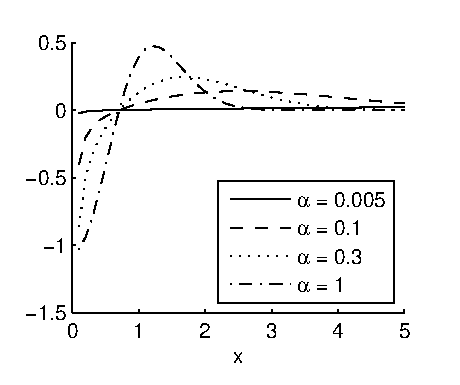
\epsfig{file=Weib-IF-mu.eps, height=2.2in} & 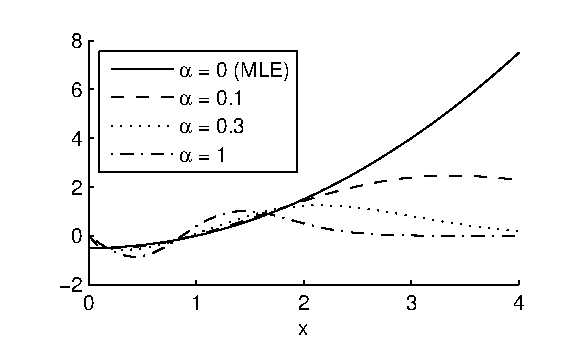
\epsfig{file=Weib-IF-lambda.eps, width=3.2in}
	\\	
	$\mathrm{IF}(x;T_{\mathfrak{R}_\alpha},\mu = 0) $, známé $\lambda = 1, \: k = 2$ & $\mathrm{IF}(x;T_{\mathfrak{R}_\alpha},\lambda = 1) $, známé $\mu = 0, \: k = 2$
\end{tabular}
\caption{Influenční funkce {\mRao}ů $\mu$ a $\lambda$ Weibullovo rozdělení}
\label{figJK:weibull-if}
\end{center}
\end{figure}

\noindent Na obrázku \ref{figJK:weibull-if} je vidět, že je influenční funkce opět omezená. V obrázku není vykreslena funkce pro $\alpha = 0$, protože pro $k=2$ je nutné použít $\alpha >0$.
Pro odhad měřítka $\theta = \lambda$ při známých $\mu, k$ má influenční funkce tvar

\begin{equation}
	\mathrm{IF}(x;T_{\mathfrak{R}_\alpha},\lambda) = \frac{(1+\alpha )^{2+\alpha -\frac{\alpha }{k}} \lambda  \left(\alpha +k (1+\alpha ) \left(-1+\left(\frac{x-\mu }{\lambda }\right)^k\right)\right)
	\left(\frac{x-\mu}{\lambda}\right)^{\alpha k-\alpha} \exp \left[-\alpha\left(\frac{x-\mu}{\lambda}\right)^k\right]}
	{k^2 \Gamma\left[2+\alpha -\frac{\alpha }{k}\right]}.
	\label{IF-weibull-lambda}
\end{equation}

\noindent Opět z použití $\Gamma$-funkce vyplývá $k>\frac{\alpha}{2+\alpha}$. Funkce pro $\alpha > 0$ a $x\rightarrow \pm \infty$ konverguje k $0$ a je omezená. což je vidět i na obrázku \ref{figJK:weibull-if}. Pro odhad parametru $\theta = k$ jsme influenční funkci opět počítali ve \texttt{Wolfram Mathematica}. Funkce vyšla ve tvaru

\begin{eqnarray}
	\mathrm{IF}(x;T_{\mathfrak{R}_\alpha},k)& = &\left(k^2 (1+\alpha )^{2+\alpha -\frac{\alpha }{k}} \left(e^{-\left(\frac{x-\mu }{\lambda }\right)^k} \left(\frac{x-\mu }{\lambda }\right)^{-1+k}\right)^{\alpha } \right. \nonumber \\
	&& \left(\alpha  \text{ln}[1+\alpha ]+k \left(1-k (1+\alpha ) \left(-1+\left(\frac{x-\mu }{\lambda }\right)^k\right)\right.\right. \nonumber \\
	&& \left.\left.\left.\left.\text{ln}\left[\frac{x-\mu }{\lambda }\right]\right)-\alpha  \psi\left[0,1+\alpha -\frac{\alpha }{k}\right]\right)\right)\right/ \nonumber \\
	&& \left(\Gamma\left[1+\alpha -\frac{\alpha }{k}\right] (k (k+\ln[1+\alpha ] \right.  \\
	&& (-2 k+2 \alpha +(k+(-1+k) \alpha ) \ln[1+\alpha ]))-2 k (-k+\alpha + \nonumber \\
	&& (k+(-1+k) \alpha )\ln[1+\alpha ]) \psi\left[0,1+\alpha -\frac{\alpha }{k}\right]+k (k+(-1+k) \alpha ) \nonumber \\
	&& \left.\left.\psi\left[0,1+\alpha -\frac{\alpha }{k}\right]^2+\left(k^2+(-1+k) k \alpha +\alpha ^2\right) \psi\left[1,1+\alpha -\frac{\alpha }{k}\right]\right)\right), \nonumber
	\label{IF-weibull-k}
\end{eqnarray}

\noindent kde $\psi(n,z)$ je $(n+1)-$tá derivace logaritmu $\Gamma(z)$, tedy

\begin{equation}
	\psi(n,z) = \frac{\mathrm{d}^{n+1}}{\mathrm{d}z^{n+1}} \ln \Gamma(z).
\end{equation}

\noindent Kvůli použití $\Gamma$-funkce vzniká podmínka $k > \frac{\alpha}{1+\alpha}$. Funkce je pro $\alpha>0$ opět omezená a pro $x$ rostoucí nade všechny meze konverguje k 0. Na obrázku \ref{figJK:weibull2-if} je patrné, že tento odhad bude fungovat kvůli velké absolutní hodnotě influenční funkce lépe pro větší hodnoty $\alpha$.

\begin{figure}[htb]
\begin{center}
\begin{tabular}{cc}	
	\multicolumn{2}{c}{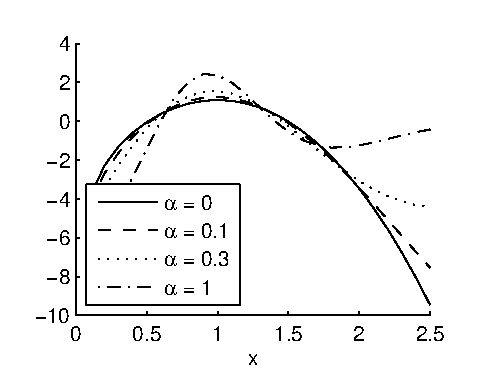
\epsfig{file=Weib-IF-k.eps, height=2.5in}}
	\\
	\multicolumn{2}{c}{$\mathrm{IF}(x;T_{\mathfrak{R}_\alpha},k = 2) $, známé $\mu = 0, \: \lambda = 1$}
\end{tabular}
\caption{Influenční funkce {\mRao}u $k$ pro Weibullovo rozdělení}
\label{figJK:weibull2-if}
\end{center}
\end{figure}



 




